\documentclass[11pt,a4paper]{scrartcl}
\usepackage[utf8]{inputenc}
\usepackage[british]{babel}
\usepackage{amsmath}
\usepackage{amsfonts}
\usepackage{amssymb}
\usepackage[headsepline]{scrlayer-scrpage}
\usepackage{minted}
\usepackage{tabu}
%\usepackage{longtable}
\usepackage{multirow}
\usepackage{setspace}
\usepackage{graphicx}
\usepackage{pgfplots}
\usepackage{hyperref}
\usepackage{url}
\usepackage{titling}
%\usepackage[backend=biber,sorting=none]{biblatex}
\usepackage{csquotes}
%\usepackage{pdfpages}
%\usepackage{epstopdf}
\usepackage{graphicx}
\usepackage{subfig}
\usepackage{siunitx}

%\usepackage{enumitem}

\pgfplotsset{width=12cm,height=6cm,compat=1.11}

% Constants
\def\mytitle{Operating Systems - Practical \#{}2}
\def\myauthor{Sébastien Vaucher}

\pagestyle{scrheadings}
\posttitle{\end{center}\begin{center}\LARGE Process Scheduling\end{center}}

\author{\myauthor}
\title{\huge \textbf{\mytitle}}

\ihead{\mytitle}
\ohead{\myauthor}

\sisetup{round-mode=places}

\begin{document}

\maketitle

\section*{Introduction}

This report is the result of the second practical project of the course Operating Systems taught at the University of Neuchâtel. The goal is to compare the performances of various process scheduling algorithms in certain conditions. To obtain data relative to the algorithms, we will use a process scheduling simulator developed at the University of Texas at San Antonio.

\section*{T1 - Individual Workload}

In this first task, we simulate a certain type of workload and compare 4 algorithms for each task.

For the interactive workload, we can see from the table below that the choice of scheduler has only little effect. This is because the tasks are short and well spaced out. The SJFA algorithm is better in this case as it provides better throughput, turnaround time and waiting time. However, the improvement is not significant.

The CPU intensive workload simulates tasks similar to scientific computations. What we want is maximal CPU utilization and minimal turnaround time. We can see that Round Robin is worse for this usage compared to the other algorithms. Round Robin uses preemption, which is not needed in this case, as it would only improve the waiting time. All three other algorithms perform in exactly the same manner, which shows that they order the tasks similarly.

In the mixed load scenario, there is no clear winner between the algorithms. SJFA offers the best CPU utilization and throughput. SJF is better in terms of turnaround and waiting times. The standard deviation of the turnaround time is quite high, because a process executing only long bursts may get delayed until all processes executing shorter bursts finish their executions. Processes executing short bursts finish earlier. This is confirmed by the Gantt chart, in which we can see that processes 1 and 3 finish at 50 while the other processes finish at 100.

\begin{figure}
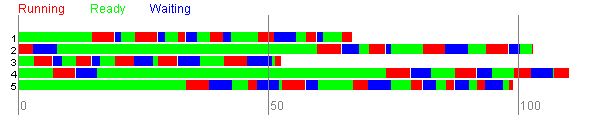
\includegraphics[width=\textwidth]{mixedload.png}
\caption{Gantt chart of mixed workload with SJF algorithm}
\end{figure}

\begin{table}
\begin{tabular}{ | l | S[round-precision=2] | S[round-precision=3] | S[round-precision=2] S[round-precision=2] | S[round-precision=2] S[round-precision=2] | }
\hline
	Workload: & \multicolumn{6}{c |}{Interactive} \\ \hline
	& & & \multicolumn{2}{c |}{turnaround time} & \multicolumn{2}{c |}{waiting time} \\
	Scheduler & {CPU util.} & {throughput} & {$\overline{x}$} & {$\sigma$} & {$\overline{x}$} & {$\sigma$} \\ \hline
	 
	FCFS & 0.678446 & 0.135689 & 32.09 & 5.32 & 3.32 & 0.1 \\ \hline
	Round Robin & 0.678446 & 0.135689 & 32.09 & 5.32 & 3.32 & 0.1 \\ \hline
	SJF & 0.678446 & 0.135689 & 32.09 & 5.32 & 3.32 & 0.1 \\ \hline
	SJFA & 0.68316 & 0.136632 & 31.62 & 5.16 & 2.85 & 0.19 \\ \hline \hline
	

	Workload: & \multicolumn{6}{c |}{CPU intensive} \\ \hline
	& & & \multicolumn{2}{c |}{turnaround time} & \multicolumn{2}{c |}{waiting time} \\
	Scheduler & {CPU util.} & {throughput} & {$\overline{x}$} & {$\sigma$} & {$\overline{x}$} & {$\sigma$} \\ \hline
	 
	FCFS & 1 & 0.25 & 180.0 & 14.14 & 135.73 & 2.52 \\ \hline
	Round Robin & 1 & 0.25 & 196.2 & 3.19 & 151.93 & 0.29 \\ \hline
	SJF & 1 & 0.25 & 180.0 & 14.14 & 135.73 & 2.52 \\ \hline	
	SJFA & 1 & 0.25 & 180.0 & 14.14 & 135.73 & 2.52 \\ \hline \hline
	

	Workload: & \multicolumn{6}{c |}{Mixed load} \\ \hline
	& & & \multicolumn{2}{c |}{turnaround time} & \multicolumn{2}{c |}{waiting time} \\
	Scheduler & {CPU util.} & {throughput} & {$\overline{x}$} & {$\sigma$} & {$\overline{x}$} & {$\sigma$} \\ \hline
	 
 	FCFS & 0.939852 & 0.046993 & 95.71 & 5.87 & 58.59 & 0.75 \\ \hline
	Round Robin & 0.960488 & 0.048024 & 98.74 & 2.73 & 61.63 & 0.35 \\ \hline
	SJF & 0.959795 & 0.04799 & 81.47 & 21.16 & 44.36 & 4.02 \\ \hline
	SJFA & 0.97665 & 0.048832 & 96.66 & 3.47 & 59.54 & 1.05 \\ \hline
	
	
\end{tabular}
\caption{T1 tables}
\end{table}

\section*{T2 - Mixing Workloads}

For the second task, we will combine processes doing interactive work with processes executing CPU intensive work. This is a scenario that is likely to happen on a desktop computer. The goal is to finish the CPU intensive tasks fast while giving priority to the interactive processes to keep the user interface responsive.

FCFS is clearly not adapted for this scenario. Problems start when a long task arrives slightly before a shortest one. The short task will have to wait for the longest task to finish before being allocated to the processor. It can get even worse if multiple long tasks are already waiting when a short task arrives.

SJF performs quite well in our simulation. Due to its priority model, short bursts never wait too long and execute in one block. In a real case, however, tasks that are CPU intensive might get starved.

SJFA is worse because the estimation of the length of bursts is imperfect. It might think that a burst is short, but is in reality long. The same problems that we have with FCFS will then appear.

Round Robin gets good statistics. The fact that it is preemptive allows interleaving of short and long bursts. Turnaround and waiting times are on par with SJF, but with higher standard deviation. Its main advantage is the lack of starvation.

\begin{table}
\begin{tabular}{ | l | S[round-precision=2] | S[round-precision=3] | S[round-precision=2] S[round-precision=2] | S[round-precision=2] S[round-precision=2] | }
\hline
	Workload: & \multicolumn{6}{c |}{Interactive \&{} CPU intensive} \\ \hline
	& & & \multicolumn{2}{c |}{turnaround time} & \multicolumn{2}{c |}{waiting time} \\
	Scheduler & {CPU util.} & {throughput} & {$\overline{x}$} & {$\sigma$} & {$\overline{x}$} & {$\sigma$} \\ \hline
	 
	FCFS & 0.977120 & 0.043428 & 208.88 & 21.32 & 171.55 & 2.91 \\ \hline
	Round Robin & 1 & 0.044444 & 152.3 & 69.62 & 114.97 & 6.1 \\ \hline
	SJF & 1 & 0.044444 & 150.9 & 55.49 & 113.57 & 4.68 \\ \hline
	SJFA & 1 & 0.044444 & 165.1 & 41.61 & 127.77 & 3.33 \\
	
\hline
\end{tabular}
\caption{T2 tables}
\end{table}

\section*{T3 - Varying the Round Robin Time Slice}

The goal of the third task is to observe the influence of the time slice parameter of the Round Robin scheduling algorithm. First we will ignore the context-switch time, and then we will redo the experiment taking it into account. The time slice defines how long a process can occupy the CPU before being preempted. A short time slice provides a fair share of CPU time to each process, at the expense of more context switches. This will have a bigger influence in the second variant of the experiment.

When we do not take context switches time into account, we can see that the time slice has minor influence towards the execution statistics. In the interactive workload, the tasks are short. Setting the time slice too low make short bursts appear longer than they really are. This introduces unnecessary waiting times, which gives poor results. Apart from the extreme $0.1$ value, all other values produce exactly the same result.

In a CPU intensive environment, Round Robin has the ability to max out the CPU utilization. The best times are obtained with higher time slices. Too high time slices are not good in terms of turnaround time, but decrease the time spent waiting.

Mixed load scenario is where Round Robin is a sensible choice. Bursts of different lengths are interleaved which permits good turnaround times. The best time slice in this case is $>5$ if we want to optimize execution times, but a small time slice provides better CPU utilization and throughput. The length of bursts in this scenario is between $1$ and $5$. We can see on the table that a good compromise utilization/time lies with a time slice in the order or the bursts length.

When context switch time is taken into account, smaller time slice values cause more preemption, leading to a decrease in efficiency. In our case, the highest value consistently produces the best statistics. For recall, the higher the time slice, the more we tend to FCFS. The advantage of Round Robin is to prevent a very long process to monopolise the CPU. The time slice has to be longer than the majority of bursts, but still permit small burst to execute without waiting too much.

\begin{table}
\begin{tabular}{ | l | S[round-precision=2] | S[round-precision=3] | S[round-precision=2] S[round-precision=2] | S[round-precision=2] S[round-precision=2] | }
\hline
	Workload: & \multicolumn{6}{c |}{Interactive} \\ \hline
	& & & \multicolumn{2}{c |}{turnaround time} & \multicolumn{2}{c |}{waiting time} \\
	Time slice & {CPU util.} & {throughput} & {$\overline{x}$} & {$\sigma$} & {$\overline{x}$} & {$\sigma$} \\ \hline

	0.1 & 0.657604 & 0.131521 & 33.47 & 4.99 & 4.70 & 0.14 \\ \hline
	0.5 & 0.678446 & 0.135689 & 32.09 & 5.32 & 3.32 & 0.10 \\ \hline
	1 & 0.678446 & 0.135689 & 32.09 & 5.32 & 3.32 & 0.10 \\ \hline
	5 & 0.678446 & 0.135689 & 32.09 & 5.32 & 3.32 & 0.10 \\ \hline
	10 & 0.678446 & 0.135689 & 32.09 & 5.32 & 3.32 & 0.10 \\ \hline \hline

	Workload: & \multicolumn{6}{c |}{CPU intensive} \\ \hline
	& & & \multicolumn{2}{c |}{turnaround time} & \multicolumn{2}{c |}{waiting time} \\
	Time slice & {CPU util.} & {throughput} & {$\overline{x}$} & {$\sigma$} & {$\overline{x}$} & {$\sigma$} \\ \hline

	0.1 & 1 & 0.25 & 197.4 & 2.84 & 153.13 & 0.12 \\ \hline
	0.5 & 1 & 0.25 & 197.0 & 2.74 & 152.73 & 0.09 \\ \hline
	1 & 1 & 0.25 & 169.20 & 3.19 & 151.93 & 0.29 \\ \hline
	5 & 1 & 0.25 & 190.0 & 7.07 & 145.73 & 1.13 \\ \hline
	10 & 1 & 0.25 & 180.0 & 14.14 & 135.73 & 2.52 \\ \hline \hline

	Workload: & \multicolumn{6}{c |}{Mixed load} \\ \hline
	& & & \multicolumn{2}{c |}{turnaround time} & \multicolumn{2}{c |}{waiting time} \\
	Time slice & {CPU util.} & {throughput} & {$\overline{x}$} & {$\sigma$} & {$\overline{x}$} & {$\sigma$} \\ \hline

	0.1 & 0.966033 & 0.048302 & 98.7 & 2.52 & 61.58 & 0.38 \\ \hline
	0.5 & 0.942695 & 0.047135 & 98.8 & 3.8 & 61.69 & 0.25 \\ \hline
	1 & 0.960488 & 0.048024 & 98.74 & 2.73 & 61.63 & 0.35 \\ \hline
	5 & 0.939852 & 0.046993 & 95.71 & 5.87 & 58.59 & 0.75 \\ \hline
	10 & 0.939852 & 0.046993 & 95.71 & 5.87 & 58.59 & 0.75 \\ \hline
	
\end{tabular}
\caption{T3 tables, without context switch time}
\end{table}

\begin{table}
\begin{tabular}{ | l | S[round-precision=2] | S[round-precision=3] | S[round-precision=2] S[round-precision=2] | S[round-precision=2] S[round-precision=2] | }
\hline
	Workload: & \multicolumn{6}{c |}{Interactive} \\ \hline
	& & & \multicolumn{2}{c |}{turnaround time} & \multicolumn{2}{c |}{waiting time} \\
	Time slice & {CPU util.} & {throughput} & {$\overline{x}$} & {$\sigma$} & {$\overline{x}$} & {$\sigma$} \\ \hline

	0.1 & 0.315830 & 0.063166 & 73.39 & 6.77 & 39.38 & 0.49 \\ \hline
	0.5 & 0.602998 & 0.1206 & 35.7 & 5.22 & 6.03 & 0.23 \\ \hline
	1 & 0.602998 & 0.1206 & 35.7 & 5.22 & 6.03 & 0.23 \\ \hline
	5 & 0.602998 & 0.1206 & 35.7 & 5.22 & 6.03 & 0.23 \\ \hline
	10 & 0.602998 & 0.1206 & 35.7 & 5.22 & 6.03 & 0.23 \\ \hline \hline

	Workload: & \multicolumn{6}{c |}{CPU intensive} \\ \hline
	& & & \multicolumn{2}{c |}{turnaround time} & \multicolumn{2}{c |}{waiting time} \\
	Time slice & {CPU util.} & {throughput} & {$\overline{x}$} & {$\sigma$} & {$\overline{x}$} & {$\sigma$} \\ \hline

	0.1 & 0.332779 & 0.008319 & 597.96 & 3.1 & 513.69 & 0.17 \\ \hline
	0.5 & 0.713776 & 0.017844 & 276.32 & 3.3 & 224.13 & 0.21 \\ \hline
	1 & 0.832639 & 0.020816 & 236.98 & 2.23 & 188.79 & 0.26 \\ \hline
	5 & 0.960615 & 0.024015 & 194.58 & 9.64 & 149.59 & 1.64 \\ \hline
	10 & 0.980392 & 0.024510 & 183.5 & 14.42 & 138.93 & 2.57 \\ \hline \hline

	Workload: & \multicolumn{6}{c |}{Mixed load} \\ \hline
	& & & \multicolumn{2}{c |}{turnaround time} & \multicolumn{2}{c |}{waiting time} \\
	Time slice & {CPU util.} & {throughput} & {$\overline{x}$} & {$\sigma$} & {$\overline{x}$} & {$\sigma$} \\ \hline

	0.1 & 0.326909 & 0.016345 & 300.80 & 2.81 & 243.46 & 0.31 \\ \hline
	0.5 & 0.674860 & 0.033743 & 140.65 & 3.82 & 99.32 & 0.27 \\ \hline
	1 & 0.789166 & 0.039458 & 122.21 & 2.23 & 82.87 & 0.45 \\ \hline
	5 & 0.886527 & 0.044326 & 101.21 & 6.38 & 63.55 & 0.82 \\ \hline
	10 & 0.886527 & 0.044326 & 101.21 & 6.38 & 63.55 & 0.82 \\ \hline
	
\end{tabular}
\caption{T3 tables, with context switch time}
\end{table}

\section*{T4 - High Load Performance}

The last task which we will investigate is high load performance. A large number of processes executing different workloads will compete. The order of arrival of the processes is important. In our case, processes executing smaller bursts arrive early. This means that SJF will be quite good.

What we observe is that the CPU utilization and throughput are the same for all algorithms. What changes is the turnaround and waiting times. SJF and SJFA make long bursts wait a long time which can be deducted from the fact that the standard deviation is really high. In this sense, Round Robin is more fair towards all types of processes. FCFS performance is abysmal, because he might make a very small bursts wait a very long time.

In the end, we can conclude that Round Robin provides a good compromise, preventing small bursts from waiting too long, and enabling long bursts to execute, even when a lot of smaller bursts are present.

\begin{table}
\begin{tabular}{ | l | S[round-precision=2] | S[round-precision=3] | S[round-precision=2] S[round-precision=2] | S[round-precision=2] S[round-precision=2] | }
\hline
	Workload: & \multicolumn{6}{c |}{High load combination of tasks} \\ \hline
	& & & \multicolumn{2}{c |}{turnaround time} & \multicolumn{2}{c |}{waiting time} \\
	Scheduler & {CPU util.} & {throughput} & {$\overline{x}$} & {$\sigma$} & {$\overline{x}$} & {$\sigma$} \\ \hline

	FCFS & 1 & 0.046154 & 9470.98 & 4409.99 & 9434.23 & 2.94 \\ \hline
	Round Robin & 1 & 0.046154 & 7004.79 & 4929.41 & 6968.04 & 3.28 \\ \hline
	SJF & 1 & 0.046154 & 4403.34 & 6311.79 & 4366.59 & 4.2 \\ \hline
	SJFA & 1 & 0.046154 & 6622.42 & 9310.77 & 6585.67 & 6.2 \\ \hline
	
\end{tabular}
\caption{T4 tables}
\end{table}

\end{document}